% Slide 12: Diferenças Estruturais entre Modalidades
\begin{frame}{Diferenças Estruturais entre Modalidades}
    \begin{columns}[T]
        \begin{column}{0.48\textwidth}
            \begin{center}
                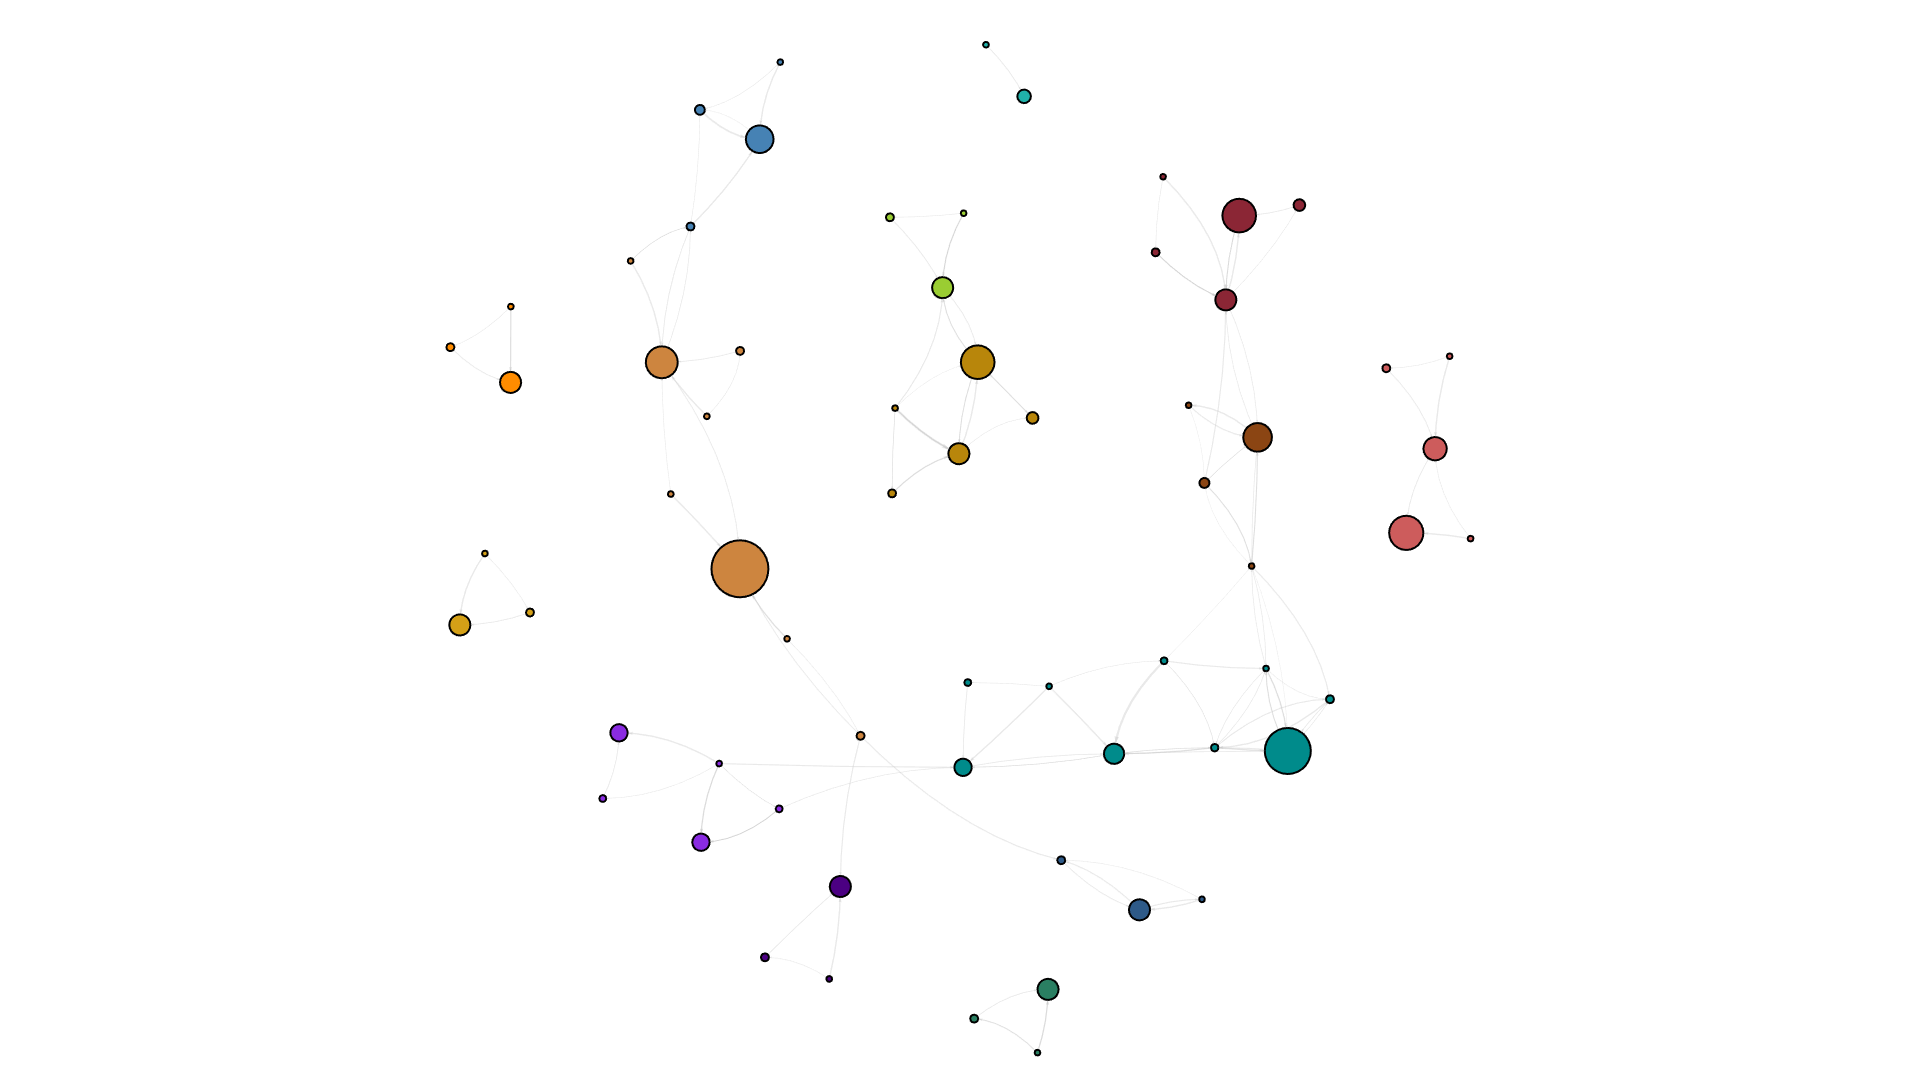
\includegraphics[width=\textwidth]{../monografia/img/swimming_M_100m.png}\\
                \vspace{0.1cm}
                \footnotesize
                \textbf{Natação 100m Livre M}\\
                Q = 0.892 --- \textit{16 eras distintas}\\
                Densidade: 5.8\%
            \end{center}
        \end{column}
        \begin{column}{0.48\textwidth}
            \begin{center}
                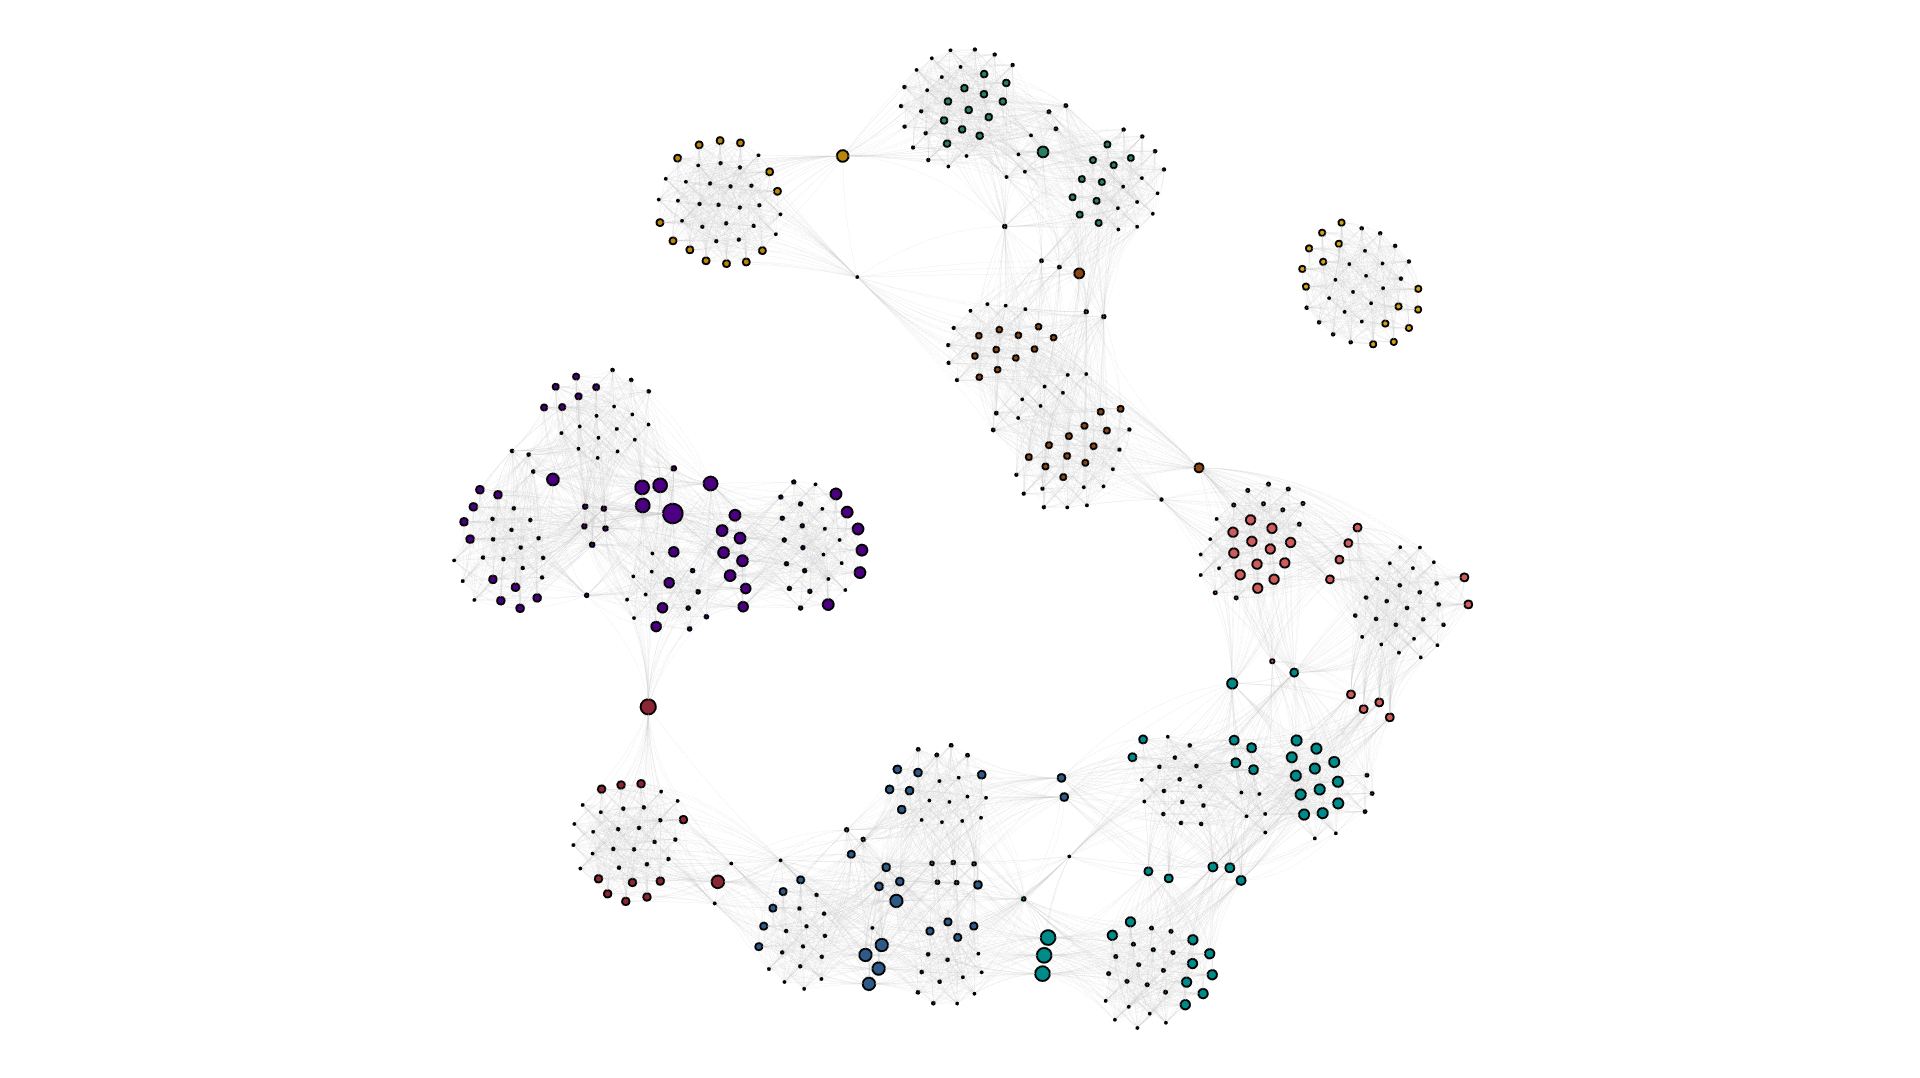
\includegraphics[width=\textwidth]{../monografia/img/basket_M.png}\\
                \vspace{0.1cm}
                \footnotesize
                \textbf{Basquete M}\\
                Q = 0.003 --- \textit{sem eras distintas}\\
                Densidade: 48.6\%
            \end{center}
        \end{column}
    \end{columns}

    \vspace{0.2cm}

    \begin{block}{Densidade: Coletivos vs Individuais}
        \footnotesize
        \begin{itemize}
            \item \textbf{Esportes Coletivos:} $\approx$ 35\% \quad \textbf{Individuais:} $\approx$ 5\% --- diferença de \textbf{7×}
            \item Cor dos nós = comunidade (era histórica) \quad Tamanho = PageRank
        \end{itemize}
    \end{block}
\end{frame}

% Slide 13: Densidade Feminina > Masculina (DESTAQUE!)
\begin{frame}{Descoberta Contra-Intuitiva: Densidade F $>$ M}
    \begin{alertblock}{Resultado Surpreendente}
        \Large
        \centering
        Redes femininas são \textbf{5.66× mais densas} que masculinas
    \end{alertblock}

    \vspace{0.5cm}

    \begin{columns}[T]
        \begin{column}{0.48\textwidth}
            \begin{block}{Razão F/M por Esporte}
                \footnotesize
                \begin{itemize}
                    \item Boxe: \textbf{25.65×}
                    \item Judô: \textbf{10.23×}
                    \item Atletismo: \textbf{5.15×}
                    \item Futebol: \textbf{5.53×}
                    \item Natação: \textbf{3.21×}
                    \item Basquete: 0.56×
                \end{itemize}
            \end{block}
        \end{column}
        \begin{column}{0.48\textwidth}
            \begin{block}{Validação Estatística}
                \footnotesize
                \begin{itemize}
                    \item Wilcoxon signed-rank test
                    \item \textbf{p = 0.031} (significativo)
                    \item Efeito genuíno
                    \item 5 de 6 esportes com F $>$ M
                \end{itemize}
            \end{block}
        \end{column}
    \end{columns}

    \vspace{0.3cm}

    \begin{center}
        \footnotesize
        \textit{Possível explicação:} menor participação histórica feminina concentra competições
    \end{center}
\end{frame}

% Slide 14: Análise de Confounders
\begin{frame}{Análise de Confounders}
    \begin{block}{Hipóteses Alternativas Testadas}
        Densidade F $>$ M poderia ser artefato de:
        \begin{itemize}
            \item Tamanho da rede (redes menores = maior densidade?)
            \item Longevidade (menos edições = maior densidade?)
            \item Tipologia esportiva (coletivo vs individual?)
        \end{itemize}
    \end{block}

    \vspace{0.3cm}

    \begin{block}{Regressão Múltipla: Controle de Confounders}
        \begin{itemize}
            \item \textbf{Modelo:} Densidade $\sim$ Gênero + Tamanho + Longevidade + Tipologia
            \item \textbf{R² = 0.91} (modelo explica 91\% da variação)
            \item \textbf{Efeito de gênero: p = 0.028} (significativo!)
            \item Tamanho, longevidade e tipologia controlados
        \end{itemize}
    \end{block}

    \vspace{0.3cm}

    \begin{alertblock}{Conclusão}
        \footnotesize
        \centering
        Densidade F $>$ M é \textbf{efeito genuíno}, não artefato metodológico
    \end{alertblock}
\end{frame}

% Slide 15: Visualização de Redes
\begin{frame}{Visualização de Redes: Futebol M vs F}
    \begin{columns}[T]
        \begin{column}{0.48\textwidth}
            \begin{center}
                \textbf{Futebol Masculino}\\
                \vspace{0.2cm}
                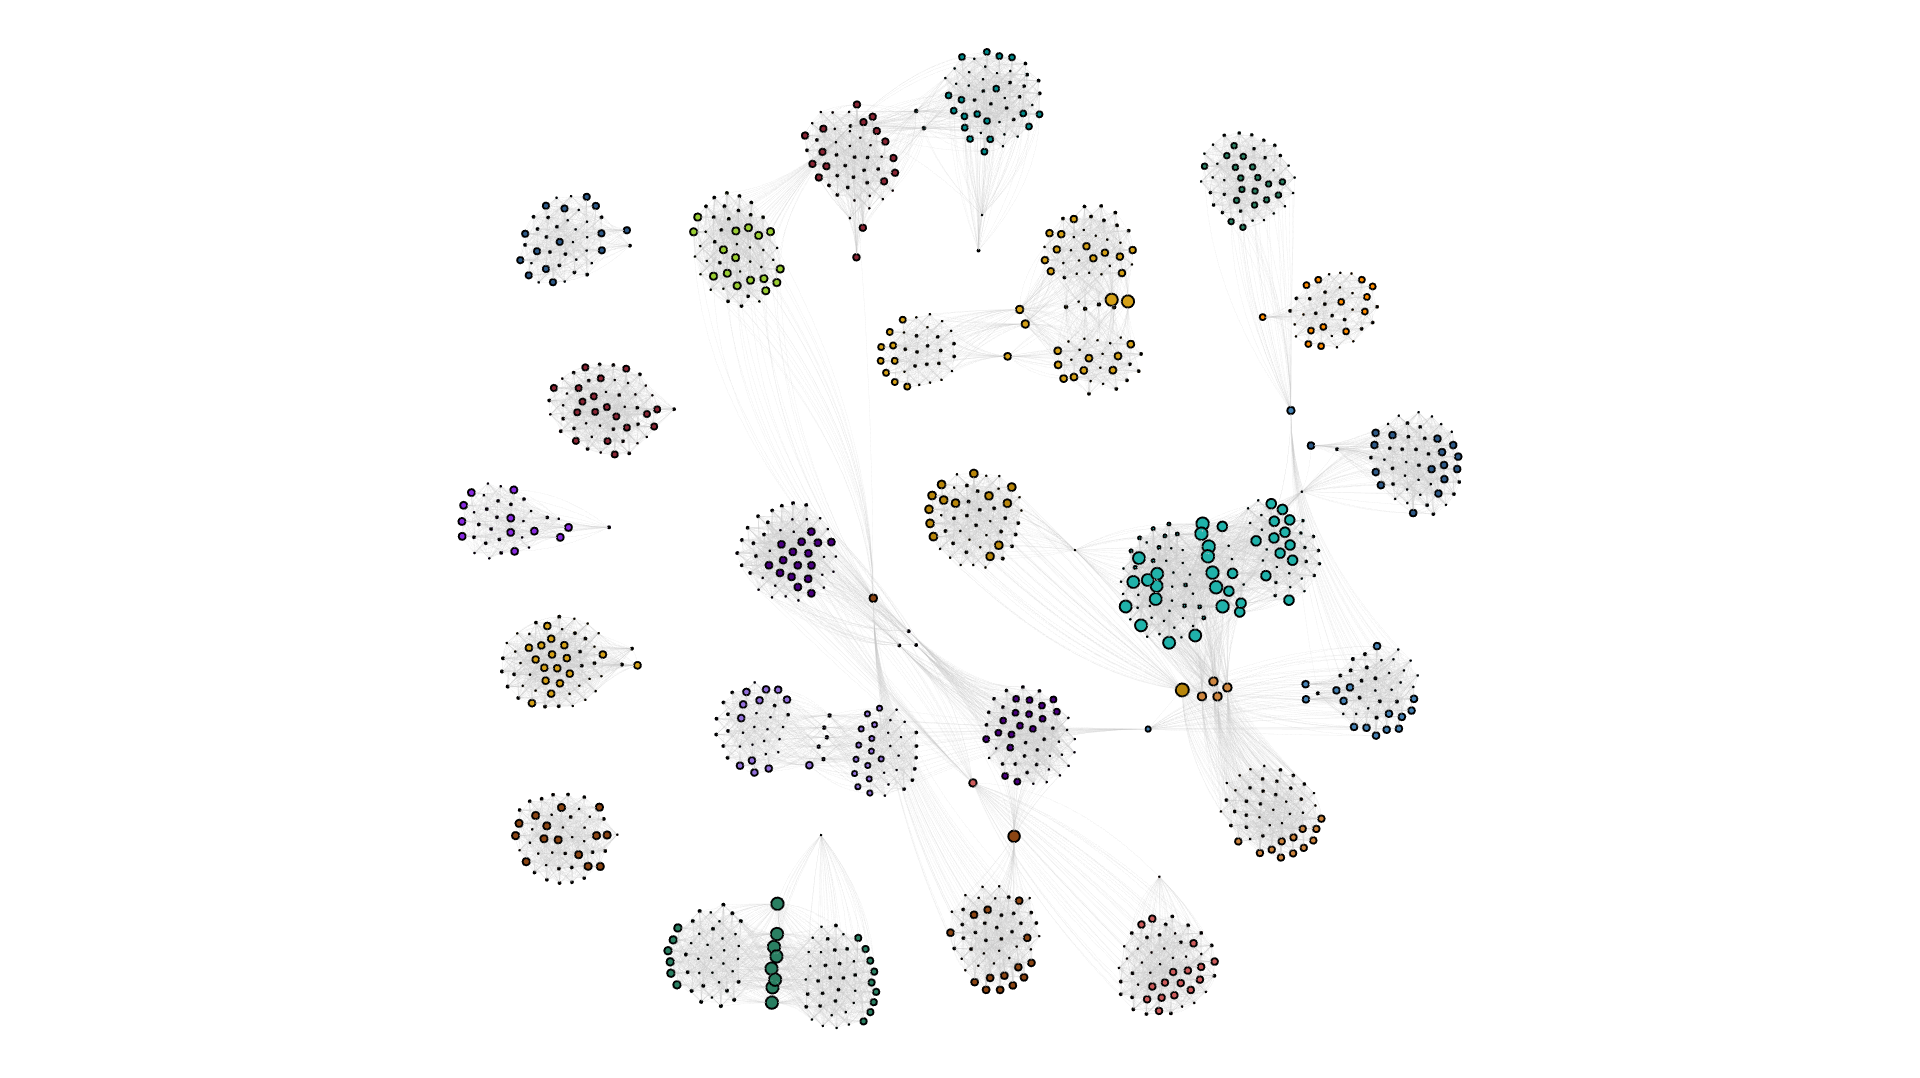
\includegraphics[width=\textwidth]{../monografia/img/futebol_M.png}\\
                \vspace{0.2cm}
                \footnotesize
                Densidade: \textbf{1.33\%}\\
                1275 atletas, 11 componentes
            \end{center}
        \end{column}
        \begin{column}{0.48\textwidth}
            \begin{center}
                \textbf{Futebol Feminino}\\
                \vspace{0.2cm}
                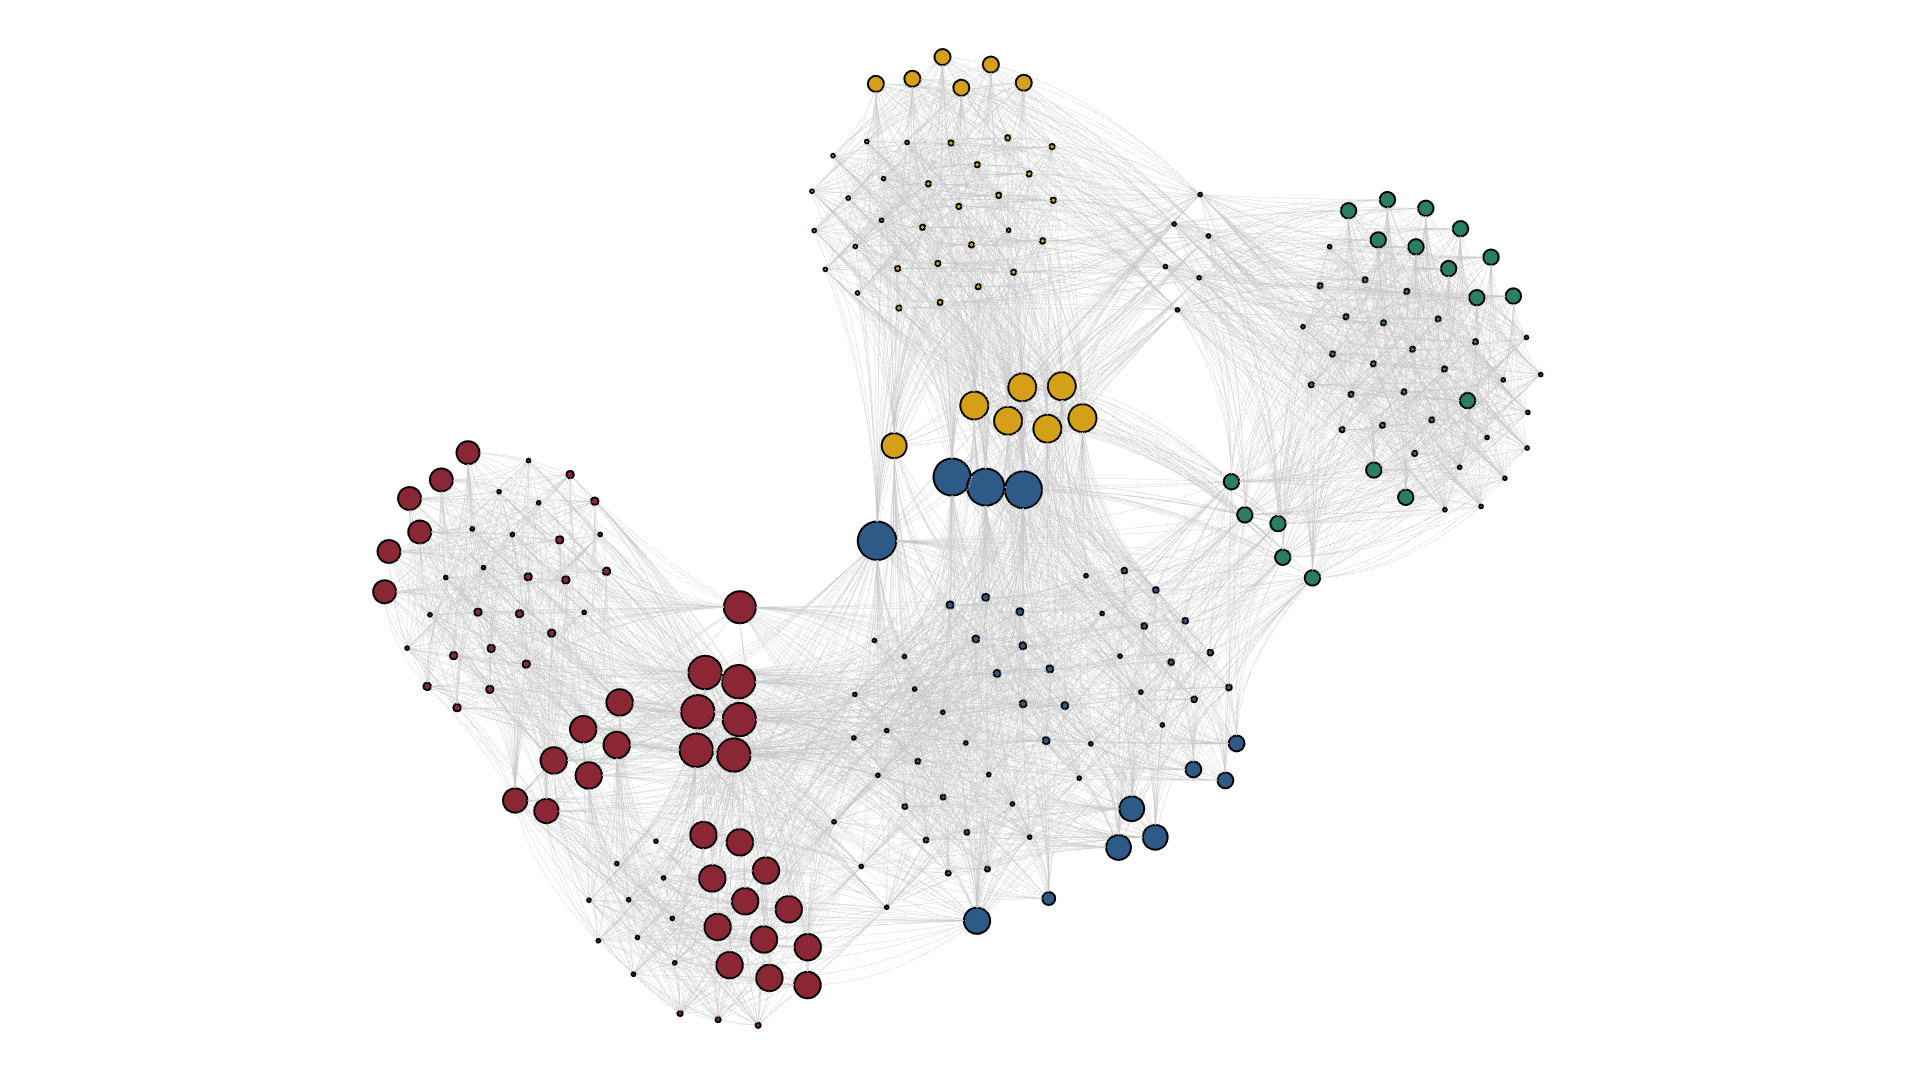
\includegraphics[width=\textwidth]{../monografia/img/futebol_F.png}\\
                \vspace{0.2cm}
                \footnotesize
                Densidade: \textbf{7.35\%}\\
                293 atletas, 2 componentes
            \end{center}
        \end{column}
    \end{columns}

    \vspace{0.3cm}

    \begin{center}
        \footnotesize
        \textbf{Razão F/M = 5.53×} -- competições femininas mais conectadas
    \end{center}
\end{frame}
